\documentclass[11pt]{report}
\usepackage{geometry}                % See geometry.pdf to learn the layout options. There are lots.
\geometry{a4paper}                   % ... or a4paper or a5paper or ...
%\geometry{landscape}                % Activate for for rotated page geometry
%\usepackage[parfill]{parskip}    % Activate to begin paragraphs with an empty line rather than an indent
\usepackage{lmodern}
\usepackage{graphicx}
\usepackage{amssymb}
\usepackage{epstopdf}
\DeclareGraphicsRule{.tif}{png}{.png}{`convert #1 `dirname #1`/`basename #1 .tif`.png}

\usepackage[colorlinks]{hyperref}
\usepackage{underscore}
\usepackage{textcomp}
\usepackage{xcolor}
\usepackage{parskip}
\usepackage{framed}
\usepackage{listings}
\usepackage[nosolutionfiles]{answers}
\usepackage{tikz}
\usetikzlibrary{arrows,automata,shapes,snakes,patterns,decorations}
\usetikzlibrary{shapes.geometric,shapes.misc}
\usetikzlibrary{shadows}
\usetikzlibrary{calc}
\usetikzlibrary{positioning}
%\usepackage{adjustbox}
\usepackage{todonotes}

\newcommand{\namedtodo}[2][]{%
% initials of the author (optional) + note in the margin
{%
\todo[color={yellow!50},size=\small]{%
\textbf{TODO [\uppercase{#1}]:}~#2}%
}}


\lstset{
  language=C,
  basicstyle=\ttfamily\footnotesize,
  commentstyle=\itshape\color{cyan},
  frame=lines
}


\Newassociation{sol}{Solution}{ans}
\newtheorem{ex}{Question}

\newcommand{\normaltilde}{{\raise.17ex\hbox{$\scriptstyle\mathtt{\sim}$}}}
\newcommand{\unixcl}[1]{\texttt{\fcolorbox{black}{gray!20}{\footnotesize#1}}}
\newcommand{\blanc}{\fcolorbox{white}{white}{~}}
\newcommand{\tabkey}{\mbox{$\rightarrow\hspace{-1.4mm}\vert$}}
\title{ETR 2021\\Lab booklet}
\author{Jean-Luc B\'echennec, Mika\"el Briday, S\'ebastien Faucou}
%\date{}                                           % Activate to display a given date or no date

\hypersetup{linkcolor=red}

\colorlet{shadecolor}{gray!10}

\begin{document}
\maketitle


\chapter{Overview}

\section{Foreword}

It is assumed that you have a basic knowledge of the command line.
If it is not the case, make sure to have the first configuration steps checked
by a member of the teaching team before to proceed with the labs.

\begin{framed}
Do not copy the commands from the PDF file, the characters you get, even if the glyph looks the same, may not have the correct code and the shell will not understand them.
\end{framed}

When typing shell commands, remember that spaces are important because they separate the command and its arguments. In this document, spaces in commands are represented by a white rectangle like in the following command (it is an example, do not type it):

\noindent
\begin{minipage}{.25\textwidth}
\unixcl{cd\blanc{}trampoline}
\end{minipage}
\begin{minipage}{.7\textwidth}
sets the \texttt{trampoline} directory as current directory. This assumes the \texttt{trampoline} directory is a subdirectory of the current one.
\end{minipage}

\section{Setting up the environment}

The tools that we will use have already been installed on the machine:

\begin{itemize}
  \item Trampoline RTOS and the \texttt{goil} configuration generator;

  \item \texttt{arm-none-eabi-gcc toolchain} including among other tools a c
    compiler and a c debugger;

  \item \texttt{stlink}, a set of tools to interact with the STM32F303 microcontroller.
\end{itemize}


Trampoline is installed in \unixcl{/opt/trampoline}. \texttt{goil} configuration generator is installed in \unixcl{/usr/local/bin}. The toolchain and \texttt{stlink}, the tool used to download binaries on the board, are installed in \unixcl{/opt}. All the usefull paths are set in the \unixcl{.bashrc} startup file of your account.

%In order to be able to use the tools, you have to define the configuration of your development environment.
%First, you have to inform the system of the location of the tools.
%This is done by setting the \texttt{PATH} environment variable in your \texttt{.profile} file.
%\namedtodo[JLB]{Update path to reflect new locations}It can be done with the following commands:
%
%\unixcl{echo\blanc{}"export\blanc{}PATH=/Volumes/PRETS/trampoline/goil/makefile-macosx:\$PATH" \blanc{}>>\blanc{}\normaltilde/.profile}
%
%
%\unixcl{echo\blanc{}"export \blanc{}PATH=/Volumes/PRETS/gcc-arm-none-eabi-8-2018-q4-major/bin:\$PATH"\blanc{}>>\blanc{}\normaltilde/.profile}
%
%To get the \normaltilde~character on french apple keyboard, you have to use Alt+n.
%
%It is assumed that the location of the\texttt{stlink} tools are already in the PATH.
%If it is not the case, update your \texttt{.profile}.
%
%The \texttt{.profile} file is parsed by the shell when it starts. To force your current shell instance to read the file, use the following command:
%
%\unixcl{source\blanc{}\normaltilde/.profile}
%
%This will enable the configuration in the terminal where you typed the command.
%In order to have the configuration active in all terminals, you have to log out and then log in the system.

Now, check that \texttt{goil} is working.
The command \unixcl{goil\blanc{}--version} should print:

\medskip

\begin{shaded*}
\scriptsize
\vspace{-1.7mm}
\begin{verbatim}
./goil : 3.1.12, build with GALGAS 3.4.3
No warning, no error.
\end{verbatim}
\end{shaded*}

Then check that \texttt{gcc-arm} is also working.
The command \unixcl{arm-none-eabi-gcc\blanc{}--version} should print:

\medskip

\begin{shaded*}
\scriptsize
\vspace{-1.7mm}
\begin{verbatim}
arm-none-eabi-gcc (GNU Arm Embedded Toolchain 10.3-2021.07) 10.3.1 20210621 (release)
Copyright (C) 2020 Free Software Foundation, Inc.
This is free software; see the source for copying conditions.  There is NO
warranty; not even for MERCHANTABILITY or FITNESS FOR A PARTICULAR PURPOSE.
\end{verbatim}
\end{shaded*}

Last, check that \texttt{stlink} tools are available with the following command: \unixcl{st-info\blanc{}--version}.
The output should be:

\medskip

\begin{shaded*}
\scriptsize
\vspace{-1.7mm}
\begin{verbatim}
v1.3.0
\end{verbatim}
\end{shaded*}

You are now ready to compile and load your first application on the board. But first, let's take a quick look at the board.

\chapter{The board}

\section{Overview}

The Master CORO lab board is built around a NUCLEO-F303K8 breakout board (BB). A breakout board is a minimal board designed to be used with tiny SMD\footnote{Surface Mounted Device} on a breadboard or in a hobbyist design. The NUCLEO-F303K8 BB is built around a ST Microelectronics microcontroller, the STM32F303K8T6, which has an ARM Cortex-M4 computing core. It is a 32 bits micro-controller running at up to 72MHz. It embeds 64kB of flash memory to store the program and the constant data and 16kB of SRAM to store the variables. Here is the NUCLEO-F303K8 BB:

\begin{figure}[htbp] %  figure placement: here, top, bottom, or page
   \centering
   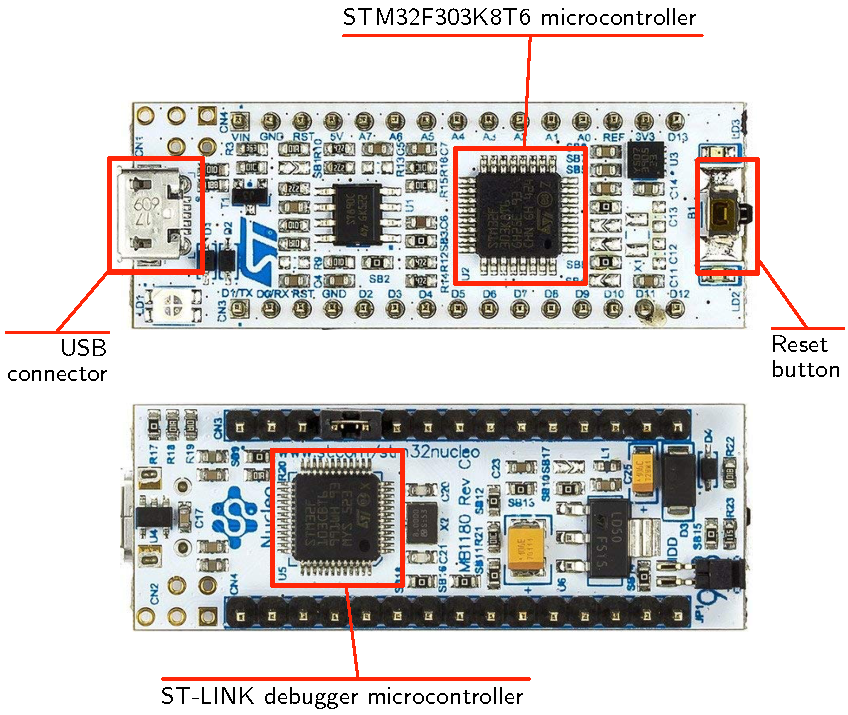
\includegraphics[scale=.7]{img/nucleo.pdf} 
   \label{fig:example}
\end{figure}


On the back, a second microcontroller runs the debugging software: ST-LINK. This software establishes a USB communication with the host development computer and allows to download your software to the STM32F303K8T6. It acts also as a JTAG debugger to do step by step execution of the software running on the STM32F303K8T6.

The NUCLEO-F303K8 is pin to pin compatible with the Arduino Nano BB but in the hearth it is very different and of course more powerful. 

\section{The Master CORO board}

The board adds the following components:
\begin{itemize}
\setlength\itemsep{-.2em}
\item{A more accessible reset button}
\item{5 push buttons}
\item{A potentiometer}
\item{A 24 pulses per turn square encoder with a push button}
\item{A 4 positions DIP-switch}
\item{1 green LED}
\item{6 red LEDs connected in charlieplexing}
\item{8 yellow LEDs}
\item{A graphical 1.8" TFT color screen}
\item{A connector for a servomotor}
\item{A connector for a unipolar stepper motor}
\item{A connector for an ultrasonic range finder}
\item{An external power supply connector}
\end{itemize}

In this list some devices are not connected to the NUCLEO-F303K8 BB but to a Microchip MCP23S17 SPI I/O expander which is an external GPIO where control and data registers are read and updated through the SPI bus: 4 of the 5 push buttons, the DIP-switch and the 8 yellow LEDs.

A picture of the board is presented at figure \ref{pic:board}

\begin{figure}[htbp] %  figure placement: here, top, bottom, or page
   \centering
   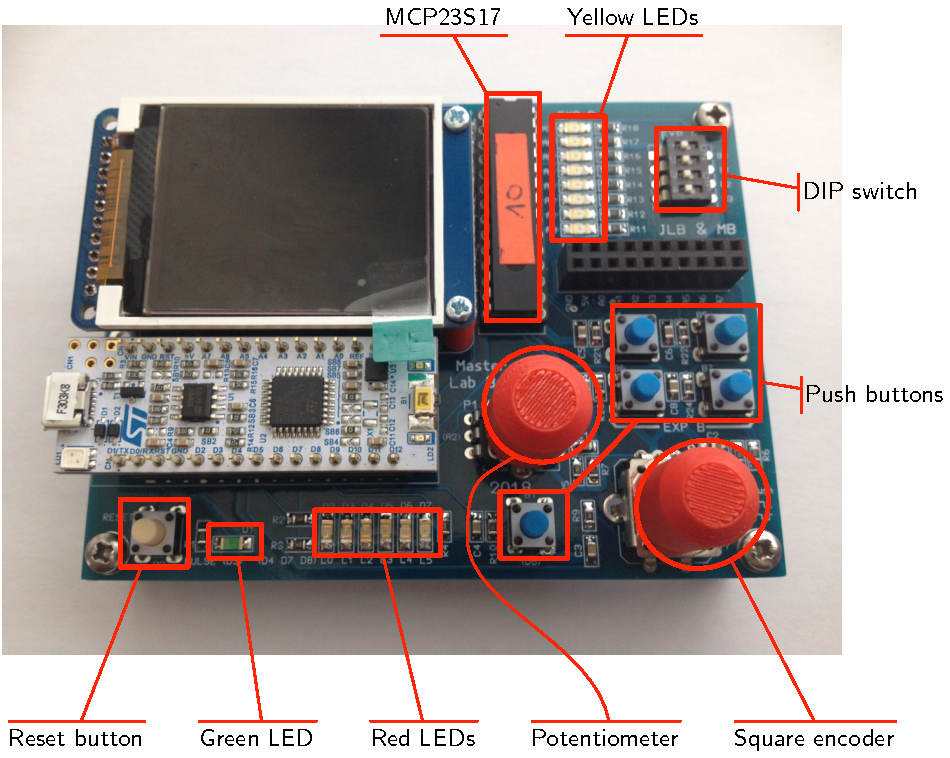
\includegraphics[scale=.7]{img/board.pdf} 
   \label{pic:board}
\end{figure}

\subsection{Reset button}

The white button in the bottom left corner of the board is the reset button. It is connected to the NUCLEO-F303K8 BB reset, to the MCP23S17 reset and to the 1.8" TFT color screen reset. The reset line is pulled up to the 3.3V supply by a 10k$\Omega$ resistor. Pressing the button pulls down the reset line to the ground.

\subsection{Push buttons}

The blue buttons are push buttons. The lone one at the bottom of the board is connected to pin D6 (Arduino)~/ PB1\footnote{Line 1 of port B.} pin of the NUCLEO-F303K8 BB. The 4 buttons on the right are connected to lines 4 to 7 of port B of the MCP23S17. Il all cases, the pull-up of the GPIO lines should be enabled and pressing the button pulls the line to the ground. Hardware debouncing is wired on all push buttons.

\subsection{Potentiometer}

The central terminal 10k$\Omega$ potentiometer is connected to the A2 (Arduino)~/ PA3~/ ADC\_IN3 pin of the NUCLEO-F303K8 BB. The two other terminals are connected to the ground and to the 3.3V supply. Turning the potentiometer clockwise decreases the voltage of this pin.

\subsection{Square encoder}

The square encoder has its push button connected to D5 (Arduino)~/~PB6 which is also the channel 4 of Timer 1. The 2 pins of the encoder are connected to A0 (Arduino)~/ PA0~/ ADC\_IN0 and A1 (Arduino)~/ PA1~/ ADC\_IN1.

\subsection{DIP switch}

The DIP switch is connected to lines 0 to 3 of port B of the MCP23S17. The pullup of this lines should be enabled. When a switch is ON, the corresponding line is pulled down to the ground.

\subsection{Green LED}

The green LED named PULSE is connected to pin D3~/ PB0~/ TIM3\_CH3. This LED is on is a high level is set on the pin.
Communication between the MCU and both the LCD and the I/O multiplexer uses the SPI interface of the MCU.
Thus to ensure integrity of transactions, the software design must enforce that transactions are atomic with regards to each others.

\section{Yellow LEDs}

8 yellow LEDs are connected to PORT A of the I/O expander. They are lit on when the line is set to the high level. 

\subsection{Power supply}

The board power is supplied by USB. Connect a USB cable to the MCU USB plug and the board switches on. If a servomotor and/or a stepper motor is connected, the green connector on the back shall be used the poser these devices.

\begin{framed}
\textbf{Note about concurrent accesses to the hardware} 

The SPI bus is shared by the TFT LCD display and the I/O expander. Concurrent accesses to the SPI bus may happen when using the functions to print on the display and/or to read/write ports of the I/O expander. In addition concurrent accesses to the display itself at higher level may happen. If more than one task use the display and/or the I/O expander, it is up to your application to protect both ressources.
\end{framed}


\section{The hardware drivers}
\label{sec:coroutils}

%\namedtodo[MB]{Update section to reflect integration of functions through
%  \texttt{setupBoard}.}{
A set of functions is provided to use the TFT LCD display, the I/O expander, and one of the embedded timer.
The source code of these functions is located within the Trampoline directory in \unixcl{machines/cortex/armv7em/stm32f303/coroLabBoard}.

Some of them are documented below. For the TFT LCD display, an object, \lstinline{Tft} is instantiated.

\begin{description}
     \item[void initCoroBoard()] initializes the GPIO and the SPI according to the hardware of the board.
%    \item[void setupIOExtender()] sets up the I/O expander. This function has to be called once, before to use the functions of the I/O Extender driver (see below).
%    \item[void setupDisplay()] sets up the display. This function has to be called once, before to use the printing functions.
    \item[void Tft.erase()] erases the TFT display.
    \item[void Tft.setTextCursor(\textit{const unsigned int col}, \textit{const unsigned int line})] set the location of the text cursor. \textit{col} argument ranges from 0 to 21 and \textit{line} argument ranges from 0 to 8.
    \item[void Tft.print(\textit{any type})] prints at the current cursor location. 
    \item[void Tft.println(\textit{any type})] same as above and goes at the beginning of the next line. 
    \item[void Tft.eraseText(\textit{const unsigned int n})] erases \textit{n} characters from the cursor location. 

%    \item[void println_string(\textit{const char * str})] prints \textit{str} on the TFT and goes to next line.
%    \item[void println_uint(\textit{uint32_t u})] prints \textit{u} on the TFT and goes to next line.
%    \item[void println_int(\textit{int32_t u})] prints \textit{i} on the TFT and goes to next line.
    \item[void setupTimer()] sets up timer TIM6 with a 1$\mu$s tick. This function has to be called once, before to use the functions related to the timer.
    \item[void resetTimer()] resets TIM6 value to 0.
    \item[uint32_t getTimerValue()] returns TIM6 current value.
\end{description}


\section{The I/O expander driver}

The I/O expander drivers implements a set of functions to change the states of LEDs and poll the state of buttons.
Notice that the programming of I/O pins in input or output is done in the \textit{setupIOExtender} function.

The driver is provided by the class \textit{mcp23s17}.
Users should not create instance of this class as a singleton instance named \textit{ioExt} is created at compile time.

Among the funciton provided by the driver, we will use:

\begin{description}
    \item[void ioExt.digitalWrite(\textit{port p}, \textit{uint8\_t bitNum, bool value})] sets the value of bit \textit{bitNum} (in the range 0 to 7) of port \textit{p} (either \texttt{mcp23s17::PORTA} or \texttt{mcp23s17::PORTB}) to value \textit{value} (0 or 1).

    \item[uint8\_t ioExt.digitalRead(\textit{port p}, \textit{uint8\_t bitNum})] returns the value of bit \textit{bitNum} (in the range 0 to 7) of port \textit{p} (either \texttt{mcp23s17::PORTA} or \texttt{mcp23s17::PORTB}).

    \item[void ioExt.digitalToggle(\textit{port p}, \textit{uint8\_t bitNum})] toggles the value of bit \textit{bitNum} (in the range 0 to 7) of port \textit{p} (either \texttt{mcp23s17::PORTA} or \texttt{mcp23s17::PORTB}).

    \item[void ioExt.setBits(\textit{port p}, \textit{uint8\_t bitField})] sets the value of bits of port \textit{p} contained in \textit{bitField} to HIGH.

    \item[void ioExt.clearBits(\textit{port p}, \textit{uint8\_t bitField})] sets the value of bits of port \textit{p} contained in \textit{bitField} to LOW.

    \item[void ioExt.writeBits(\textit{port p}, \textit{uint8\_t val})] overwrites values of bits of \textit{p} with \textit{val}.

    \item[uint8_t ioExt.readBits(\textit{port p})] returns the values of bits of \textit{p}.
\end{description}

As an illustration, the following code turn on LED 0 and toggles LED 1.

\begin{lstlisting}[language=C]
TASK(t_LED0ON_LED1TOGGLE)
{
    ioExt.digitalWrite(mcp23s17::PORTA, 0, 1);
    ioExt.digitalToggle(mcp23s17::PORTA, 1);
    TerminateTask();
}
\end{lstlisting}


And the following example reads switch button {0} to start Trampoline in a specific appmode.

\begin{lstlisting}[language=C]
int main()
{
    if (ioExt.digitalRead(mcp23s17::PORTB, 0) == 0)
    {
      /* Start Trampoline in the testAppmode appmode */
      StartOS(testAppmode);
    }
    else                       /* otherwise */
    {
      /* Start Trampoline in the default appmode */
      StartOS(OSDEFAULTAPPMODE);
    }
    return 0;
}
\end{lstlisting}


\chapter{Lab 1 -- Periodic tasks}

\section{Goal}

The goal of this lab is to become familiar with the development
process of application using Trampoline RTOS, and to understand tasks and alarms.

Trampoline includes an OIL compiler.
It reads a static description of the objects of the application (tasks,
ISRs, events, resources, etc.) and generates the corresponding OS data structures.
In addition to the OIL description, the developer must of course provide the C
source code of the body of tasxISRs.


\section{Starting point}

Go into the lab1 directory. There are 2 files:

\begin{description}
    \item[lab1.oil] a minimal OIL description.
    \item[lab1.cpp] a minimal source code.
\end{description}

Edit the lab1.oil file and update the \texttt{TRAMPOLINE\_BASE\_PATH} attribute
in function of your configuration: it should point to the directory where Trampoline is installed.

%You should also modify the \texttt{LDFLAGS} lines describing the location of the libraries used by the cross compiler. Set the first line to:

%{\footnotesize
%\begin{verbatim}
%-L/usr/local/tp_treel_imta/gcc-arm-none-eabi-7-2018-q2-update/arm-none-eabi/lib/thumb/v7e-m
%\end{verbatim}}

%and the second one to:

%{\footnotesize
%\begin{verbatim}
%-L/usr/local/tp_treel_imta/gcc-arm-none-eabi-7-2018-q2-update/lib/gcc/arm-none-eabi/7.3.1/thumb/v7e-m
%\end{verbatim}}


lab1 is a very simple application with only 2 tasks named \texttt{task1} and \texttt{pulse}. \texttt{task1}
starts automatically (\texttt{AUTOSTART = TRUE \{ ... \}} in the OIL file) and
turns on LED A0. \texttt{pulse} is activated by an alarm, \texttt{alarm\_pulse}, every 250 ms. \texttt{pulse} toggles the LED named PULSE and display a count on the LCD. Examine the OIL file and the source file.

To compile this application, go into the lab1 directory and type (on a single line):

%\unixcl{\parbox{230\unitlength}{export\blanc{}PATH=\$PATH\textbackslash\\
%:\normaltilde/trampoline/goil/makefile-macosx\textbackslash\\
%:\normaltilde/Tools/gcc-arm/gcc-arm-none-eabi/bin\textbackslash\\
%:\normaltilde/Tools/bin}}

%\namedtodo[JLB]{update path}
\unixcl{\parbox{\linewidth}{%
        goil\blanc{}--target=cortex/armv7em/stm32f303/coroLabBoard\blanc{}lab1.oil}}

The \texttt{--target} option is used to define the target system (here we generate the OS level data structures of Trampoline for a \texttt{cortex} core with the \texttt{armv7em} instruction set, a \texttt{stm32f303} micro-controller and the board is the \texttt{coroLabBoard}).
%The \texttt{--templates} option indicates where to find the template files used to generate the configuration of the kernel.

Alongside the C files of the kernel configuration, Goil also generates a build script for the application (files \texttt{make.py} and \texttt{build.py}).

If you change something in the OIL file or in your source code file, you do not need to re-run Goil because the build script should run it when needed.

Continue the build process by typing:

\unixcl{./make.py}

The application and Trampoline OS are compiled and linked together.
The target file is named \texttt{lab1.elf}.

To upload the application, check that the board is connected to the computer, then type:

\unixcl{./make.py\blanc{}burn}

The following message is displayed (some lines have been truncated to fit on the page and the version of st-flash may differ):

\begin{shaded*}
\scriptsize
\vspace{-1.7mm}
\begin{verbatim}
Nothing to make.
st-flash write lab1.elf.bin 0x8000000
st-flash 1.5.1
2019-04-28T17:45:53 INFO common.c: Loading device parameters....
2019-04-28T17:45:53 INFO common.c: Device connected is: F334 device, id 0x10016438
2019-04-28T17:45:53 INFO common.c: SRAM size: 0x3000 bytes (12 KiB), Flash: 0x10000 ...
2019-04-28T17:45:53 INFO common.c: Attempting to write 16660 (0x4114) bytes to stm32 ...
Flash page at addr: 0x08004000 erased
2019-04-28T17:45:53 INFO common.c: Finished erasing 9 pages of 2048 (0x800) bytes
2019-04-28T17:45:53 INFO common.c: Starting Flash write for VL/F0/F3/F1_XL core id
2019-04-28T17:45:53 INFO flash_loader.c: Successfully loaded flash loader in sram
  9/9 pages written
2019-04-28T17:45:53 INFO common.c: Starting verification of write complete
2019-04-28T17:45:54 INFO common.c: Flash written and verified! jolly good!
\end{verbatim}
\end{shaded*}

The program starts (if it do not start press the reset button) and:
\begin{itemize} 
\item LED A0 should be on;
\item LED PULSE should blink;
\item A number should increment in the upper left corner of the LCD.
\end{itemize}

%\subsection{A word about memory sections}

%AUTOSAR defines a way to put objects (constants, variables and functions) in memory sections in a portable way\footnote{memory section declaration is not part of the C standard}. For that, a set of macro are used along with a generated file: MemMap.h. Functions should be declared with the \lstinline{FUNC} macro, variables with the \lstinline{VAR} macro, constants with the \lstinline{CONST} macro and pointers to variables, pointers to constant, constant pointers to variable and constant pointers to constant with \lstinline{P2VAR}, \lstinline{P2CONST}, \lstinline{CONSTP2VAR} and \lstinline{CONSTP2CONST} respectively. Sections are opened and closed with a macro definition and the inclusion of the \lstinline{tpl_memmap.h} file. For instance:

%\begin{lstlisting}
%#define APP_Task_my_periodic_task_START_SEC_VAR_32BIT
%#include "tpl_memmap.h"
%VAR(int, AUTOMATIC) period;
%VAR(int, AUTOMATIC) occurence;
%#define APP_Task_my_periodic_task_STOP_SEC_VAR_32BIT
%#include "tpl_memmap.h"
%\end{lstlisting}

%defines variables \lstinline{period} and \lstinline{occurence} in the variables section of task \lstinline{my_periodic_task}.

%\begin{lstlisting}
%#define APP_Task_my_periodic_task_START_SEC_CODE
%#include "tpl_memmap.h"
%TASK(my_periodic_task)
%{
  %...
  %TerminateTask();
%}
%#define APP_Task_my_periodic_task_STOP_SEC_CODE
%#include "tpl_memmap.h"
%\end{lstlisting}

%defines the task \lstinline{my_periodic_task} in the code section of task \lstinline{my_periodic_task}. \lstinline{goil} generates the sections for tasks according to the description.


\section{First add-on}

Add a 3rd task identical to the pulse task (except for the name which is pulse2) and an alarm with offset 250 and period 50. This pulse2 task toggles the LED A7.

\section{Second add-on}

Replace the code of the pulse2 task by the code you find in the lab1-add-on directory (this directory is at the same level as lab1).

\section{Third add-on}

Instead of changing the state of LED A3, cancel or start the alarm_pulse. Refer to the OSEK QRDC. You need the GetAlarm, CancelAlarm and SetRelAlarm services.



%\subsubsection{Using the debugger to follow the scheduling}
%\namedtodo[SF]{add text on gdb, add \texttt{init.gdb}
%  in code.}{TODO}
%
%\begin{ex}
%  Run the application step by step with the debugger and follow the scheduling.
%  Identify precisely the preemption point in the code of each tasks.
%\end{ex}

%
%\subsubsection{Measuring execution times with a timer}
%
%%\namedtodo[SF]{add text on timer API + text on where to use functions}{TODO}
%
%\begin{ex}
%    Build an application to measure the execution time of \texttt{ActivateTask} in the following cases:
%    \begin{itemize}
%        \item fully preemptive scheduling, activation of a higher priority task.
%        \item fully preemptive scheduling, activation of a lower priority task.
%        \item fully non preemptive scheduling, activation of a higher priority task.
%        \item fully non preemptive scheduling, activation of a lower priority task.
%    \end{itemize}
%
%    Explain how to use the timer functions for each case and explain the results.
%\end{ex}
%
%\subsection{Task chaining}
%
%The \texttt{ChainTask()} system call allows to chain the execution of a task: the calling job terminates and a new job of the target task is created.
%
%\begin{ex}
%    Starting from the application of question~1, replace the call to \texttt{TerminateTask} by a \texttt{ChainTask(task3)} at the end of task a task.
%    Update task \texttt{task3} so that it prints something each time it is executed.
%    Draw a schedule of the new system.
%    Then execute the application to check the correctness of your diagram.
%    Comment on the differences with the previous application.
%\end{ex}
%
%\begin{ex}
%    Chain to \texttt{task2} instead of \texttt{task3}.
%    Update task \texttt{task2} so that it prints something each time it is executed.
%    Draw a schedule of the new system.
%    Then execute the application to check the correctness of your diagram.
%    Comment on the differences with the previous application.
%\end{ex}
%
%\begin{ex}
%    Test the error code returned by ChainTask.
%    Modify the OIL file so that ChainTask returns \texttt{E\_OK}.
%    Draw a schedule of the new system.
%    Then execute the application to check the correctness of your diagram.
%    Comment on the differences with the previous application.
%\end{ex}
%
%\begin{ex}
%    Build an application to measure the execution time of \texttt{ChainTask} in the following cases:
%    \begin{itemize}
%        \item fully preemptive scheduling, activation of a higher priority task.
%        \item fully preemptive scheduling, activation of a lower priority task.
%        \item fully non preemptive scheduling, activation of a higher priority task.
%        \item fully non preemptive scheduling, activation of a lower priority task.
%    \end{itemize}
%
%    Explain how to use the timer functions for each case and explain the results.
%\end{ex}
%
%\section{Extended tasks and synchronization using events}
%
%\textcolor{red}{\emph{For the following exercises, you should use full preemptive scheduling mode.}}
%
%Unlike a basic task, an extended task may wait for an event.
%In terms of scheduling, a job is activated when a task is activated or when it leaves the waiting state.
%
%Before to proceed with the following questions, consult the slides of the course to become familiar with events in Trampoline.
%
%%In the OIL file, set the priority of \texttt{task_0} to 8 and add two events \texttt{evt_0} and \texttt{evt_1}. \texttt{evt_0} is used by \texttt{task_0} and \texttt{evt_1} is used by \texttt{task_1}. \texttt{a_task} activates \texttt{task_0} and \texttt{task_1} then sets \texttt{evt_0} and \texttt{evt_1} and terminates. \texttt{task_0} and \texttt{task_1} wait for their event, clear it and terminate.
%
%\begin{ex}
%     Based on the application of Question~1, build an application with the following characteristics:
%\begin{itemize}
%    \item set priority of \texttt{task2} to 8 (so priorities are 1 for \texttt{task1} and 8 for both \texttt{task2} and \texttt{task3});
%    \item add two events, \texttt{evt\_2} and \texttt{evt\_3}:
%        \begin{itemize}
%            \item \texttt{evt\_2} is set by task \texttt{task1} to task \texttt{task2}.
%            \item \texttt{evt\_3} is set by task \texttt{task1} to task \texttt{task3}.
%        \end{itemize}
%    \item modify the code of the tasks:
%        \begin{itemize}
%            \item task \texttt{task1} activates \texttt{task2} and \texttt{task3} then sets \texttt{evt\_2} and \texttt{evt\_3} before to terminate.
%            \item tasks \texttt{task2} and \texttt{task3} wait for their event, clear it, and terminate.
%        \end{itemize}
%\end{itemize}
%
%Draw a schedule of the new system.
%Then execute the application to check the correctness of your diagram (before to run the application, add outputs in the code of the task, for instance writes to the LCD or LEDs to ease the correctness checking).
%
%\end{ex}
%
%\begin{ex}
%    Build an application to measure the execution time of \texttt{SetEvent} in the following cases:
%    \begin{itemize}
%        \item fully preemptive scheduling, setting an event to a higher priority tasks that is not waiting for the event.
%        \item fully preemptive scheduling, setting an event to a higher priority tasks that is waiting for the event.
%        \item fully preemptive scheduling, setting an event to a lower priority tasks that is not waiting for the event.
%        \item fully preemptive scheduling, setting an event to a lower priority tasks that is waiting for the event.
%    \end{itemize}
%
%    Explain how to use the timer functions for each case and explain the results.
%\end{ex}
%
%\begin{ex}
%Program an application conforming to the following requirements:
%
%\begin{itemize}
%    \item it is composed of two tasks: \texttt{server} priority 2, \texttt{t1} priority 1.
%    \item \texttt{server} is an infinite loop that activates \texttt{t1} and waits for event \texttt{evt\_1}.
%    \item \texttt{t1} prints ``I am t1'' and sets \texttt{evt\_1} of \texttt{server}.
%\end{itemize}
%
%Before to run the application, draw a schedule of the execution. Add outputs in the bodies of the task (for instance writes to the LCD or the LEDs) to verify your schedule.
%\end{ex}
%
%\begin{ex}
%Extend the previous application by adding 2 tasks: \texttt{t2} and \texttt{t3} (priority 1 for both) and 2 events \texttt{evt\_2} and \texttt{evt\_3}. \texttt{server} activates \texttt{t1}, \texttt{t2} and \texttt{t3} and waits for one of the events. When one of the events is set, \texttt{server} activates the corresponding task again.
%
%Before to run the application, draw a schedule of the execution. Add outputs in the bodies of the task (for instance writes to the LCD or the LEDs) to verify your schedule.
%\end{ex}
%
%%================================================================
%\chapter{Lab 2 -- Periodic tasks and Alarms}
%
%\section{Goal}
%
%Real-Time systems are reactive systems which have to do processing as a result of events. You have seen in Lab \#1 how to start processing as a result of an internal event of the system: by activating a task (\texttt{ActivateTask} and \texttt{ChainTask} services) or by setting an event (\texttt{SetEvent} service). In this lab, you will trigger processing as a result of time elapsing (expiration of an Alarm). This lab uses the following concepts: alarm and counter. On the lab board, the Systick timer is used as interrupt source for alarms. The interrupt is sent every 1ms.
%
%\section{First application}
%
%This application implements a periodic task that reads switch button B0 of the board every 100ms.
%When switch B0 is open, A3 is turned off.
%When button B0 is closed, A3 is turned on.
%
%\begin{ex}
%    The \texttt{updateStateOfB0} function implements a small state machine to convert the state of the switch button to states and events.
%    Draw this state machine.
%    Draw a schedule of the application (the execution of the interrupt service routine associated with the Systick will not be represented; it will be assumed to be negligible).
%    Your diagram should show the instants where the state of the switch changes as well as the state of A3.
%    Build and execute the application to verify your diagram.
%\end{ex}
%
%Modify the application: when B0 is closed, a processing is triggered.
%This processing is performed by activating a job of task \texttt{t_process} (priority 3) that, on odd executions, turns on LEDS A4 to A8 and on even executions turns them off.
%\begin{ex}
%Draw a schedule of the application.
%Your diagram should show the physical state of the switch as well as the state of the LEDs (associate numbers with the different state and use these numbers in your diagram).
%Build and execute the application to verify your diagram.
%\end{ex}
%
%
%\section{Second application}
%
%The second application will use 2 periodic tasks: \texttt{t1} (priority 2, period 1s) and \texttt{t2} (priority 1, period 1.5s). t1 toggles LED A3 each time it executes and t2 toggles LED A4.
%
%\begin{ex}
%    Draw a schedule of the application that show the 20 first states of the LEDs.
%    What is the global period of the system?
%\end{ex}
%
%The application needs a counter and 2 alarms. Program, build, and run the application.
%
%\section{Third application}
%
%In the third application, alarms, counters, and polling of the switch buttons are mixed.
%This application is a system with 2 switches.
%After startup, the system is waiting.
%When the first switch is closed, the system starts a {\it function}\footnote{Here we mean a function of the application, not a function of the C language.} F that is implemented using a periodic task (period = 1s).
%To ``see'' F, uses a blinking LED.
%When the first switch is opened, function F is stopped.
%When the second switch is closed, the system is shutdown as quickly as possible (ie ShutdownOS\footnote{The ShutdownOS service shutdowns the operating system. All tasks and alarms are stopped. ShutdownOS takes a StatusType argument to specify the kind or error which occurred. In our case use E\_OK as argument.} is called).
%
%\begin{ex}
%    Explain the design of the application: provide the list and configuration of tasks and alarms.
%    Draw schedules showing different executions.
%    Build and execute the application to verify your diagrams.
%\end{ex}
%
%Requirements change. Now function F implementation needs an Init code
%(runs once when F is started) and a Final code (runs once when F is stopped) as shown in the following diagram:
%
%\begin{center}
%    \resizebox{14cm}{!}{%
%\begin{tikzpicture}
%\draw[step=.5cm,gray!20,very thin] (-0.5, -0.5) grid (16.5,1.5);
%\draw [->] (-0.5,0) -- (16,0);
%\node [yshift=-3mm] at (16,0) {time};
%\draw (0,0) rectangle (1.2,1);
%\node at (0.6,0.5) {Init};
%\draw (1.2,0) rectangle (2.7,1);
%\node at (1.95,0.5) {Body};
%\draw (4,0) rectangle (5.5,1);
%\node at (4.75,0.5) {Body};
%\draw (8,0) rectangle (9.5,1);
%\node at (8.75,0.5) {Body};
%\foreach \x in {0, 4}
%  \draw [xshift=\x cm,thick,<->] (0,-0.5) -- (4,-0.5);
%\draw [xshift=8 cm,thick,<-(] (0,-0.5) -- (3,-0.5);
%\draw [xshift=11cm] (0,0) rectangle (1.2,1);
%\node [xshift=11cm] at (0.6,0.5) {Final};
%\node [rectangle callout, fill=green!50, callout absolute pointer={(0,1)}] at (-1,2) {Start request};
%\node [rectangle callout, fill=red!50, callout absolute pointer={(11,1)}] at (12,2) {Stop request};
%\end{tikzpicture}
%} %% resizebox
%\end{center}
%
%
%\begin{ex}
%    Modify the application to take the new requirements into account.
%    Your implementation will use only basic tasks.
%    Each phase of F (Init, Body, and Final) is executed in a different task.
%    Explain the design of the application: provide the list and configuration of tasks and alarms.
%    Draw schedules showing different execution scenarii.
%    Build and execute the application to verify your diagrams.
%\end{ex}
%
%\begin{ex}
%    Same question as above, but your implementation will use an extended task to control the execution of Init, F, and Stop.
%\end{ex}
%
%\section{Fourth application}
%
%In this part, you will implement a watchdog. It is a mechanism that allows to stop a processing or a waiting period once a delay has elapsed.
%
%In your application, each time B0 is closed, B3 must be pressed within 4 seconds. In this case, you print the time between the two occurrences. Otherwise, an error message is displayed. If B0 is closed more than once are within 5 seconds from the first time, these events are ignored.
%
%\begin{ex}
%    Specify this behaviour with a state machine.
%    What is happening if the timeout occurs just after B3 has been closed but before the waiting task got the event?
%    Design and program a solution that handles this situation correctly.
%    Draw a schedule of the behaviour of your application in such a scenario (this schedule should show the state of the alarms).
%\end{ex}
%
%\section{Fifth application}
%
%Program a chase\footnote{chenillard in French} with a 0.5s period. To do so, use 8 periodic tasks. Each periodic task manages a LED. The chase effect is done by using alarms with a time shift between them.
%
%When B0 is closed, the chase starts, when it is opened, it is reset.
%When B3 is closed, the chase stops until B3 is opened.
%When B2 is closed, the chase direction changes (even if it is stopped).
%
%\begin{ex}
%    Specify the high level behaviour with a state machine.
%    Design and program the application.
%    Explain your design.
%\end{ex}
%
%%================================================================
\chapter{Lab 2 -- Critical sections : Resources}

To show resources usage, we will use a bad program that allows to corrupt a shared global variable which is not protected against concurrent writes. 

%To ensure that the compiler does not hide our bug, update the value of the \texttt{CFLAGS} key in the OIL file: replace option \texttt{-Os} by \texttt{-O0} to turn off all optimizations.

\section{Application requirements}

The diagram of figure~\ref{fig:appdiag} describes the application.
It is composed of 3 tasks that share 2 global variables {\bf declared with the volatile keyword}: \texttt{val} and \texttt{activationCount}:
\begin{itemize}
\item a background task called \texttt{bgTask} which is activated at startup. In an infinite loop it increments then decrements the global variable \texttt{val}. This task has priority 1.
\item a periodic task called \texttt{periodicTask} that activates every 1ms. This periodic task increments the global variable \texttt{activationCount}. If \texttt{activationCount} is odd, \texttt{val} is incremented, otherwise it is decremented. This task has priority 5.
\item a periodic task \texttt{displayTask} that runs every 1.5 second and prints \texttt{val} on the LCD. This task has priority 2.
\end{itemize}

\def\alarm#1#2{
  \node[alarm](#1) [#2] {};
  \coordinate (a) at ($(#1.north)$);
  \coordinate (b) at ($(#1.north east)$);
  \coordinate (c) at ($(#1.north west)$);
  \coordinate (d) at ($(#1)$);
  \draw[thick] ($(a)+(-0.1,0)$) rectangle ($(a)+(0.1,0.1)$);
  \draw[rotate=-45,thick] ($(b)+(-0.05,0)$) rectangle ($(b)+(0.05,0.1)$);
  \draw[rotate=45,thick] ($(c)+(-0.05,0)$) rectangle ($(c)+(0.05,0.1)$);
  \draw ($(d)+(0.3,0)$) -- (d) -- ($(d)+(0,0.3)$);
  \node [font=\scriptsize,below=0.5mm of #1] {{\em Alarm}}
}

\def\sharedvar#1#2#3{
  \node (#1) [#2] {#1};
  \coordinate (a) at ($(#1.north #3) + (0,0.2)$);
  \coordinate (b) at ($(#1.south #3) + (0,-0.2)$);
  \draw[ultra thick] (a) -- (b);
  \draw ($(a)+(-0.1,0)$) -- ($(a)+(0.1,0)$);
  \draw ($(b)+(-0.1,0)$) -- ($(b)+(0.1,0)$)
}

\def\varrect#1{
  \draw ($(#1.south west)$) rectangle ($(#1.north east)$)
}

\begin{figure}[htbp] %  figure placement: here, top, bottom, or page
   \centering
   \begin{tikzpicture}[
   task/.style={draw,very thick,fill=white,drop shadow={opacity=0.25},text width=2.5cm, text centered, minimum height=1.5cm},
   alarm/.style={draw,thick,circle,fill=white,drop shadow={opacity=0.25},text width=.5cm}
   ]
   \node[task](periodicTask) at (0,0) {periodicTask};
   \node[task](bgTask) [above=of periodicTask] {bgTask};
   \node[task](displayTask) [above=of bgTask] {displayTask};
   \alarm{activateDisplay}{left=20mm of displayTask};
   \alarm{activatePeriodic}{left=20mm of periodicTask};
   \sharedvar{val}{left=of bgTask}{east};
   %\sharedvar{activationCount}{right=of periodicTask}{west};
   \sharedvar{stdout}{right=of displayTask}{west};
   \varrect{stdout};
   \draw [thick,<->] (val.east) -- (bgTask.west);
   \draw [thick,->] (val.north east) -- ++(5mm,0) |- ($(displayTask.south west) + (0,2mm)$);
   \draw [thick,<->] (val.south east) -- ++(5mm,0) |- ($(periodicTask.north west) + (0,-2mm)$);

   \draw [thick,->] (activateDisplay.east) -- ++(5mm,0) -- ++(0,1.5mm) -- ++(3mm,-3mm) -- ++ (0mm,1.5mm) -- (displayTask);
   \node at ($(activateDisplay.east) + (6.5mm,-3mm)$) {2s};
   \node[font=\scriptsize] at ($(activateDisplay.east) + (9mm,3mm)$) {{\em ActivateTask}};
   \draw [thick,->] (activatePeriodic.east) -- ++(5mm,0) -- ++(0,1.5mm) -- ++(3mm,-3mm) -- ++ (0mm,1.5mm) -- (periodicTask);
   \node at ($(activatePeriodic.east) + (6.5mm,-3mm)$) {50ms};
   \node[font=\scriptsize] at ($(activatePeriodic.east) + (9mm,3mm)$) {{\em ActivateTask}};
   %\draw [thick,<->] (activationCount.west) -- (periodicTask);
   %\draw [thick,->] (activationCount.north west) -- ++(-5mm,0) |- ($(displayTask.south east) + (0,2mm)$);
   \draw [thick,->] (displayTask) -- (stdout);
   \end{tikzpicture}
   \caption{Application diagram}
   \label{fig:appdiag}
\end{figure}

Run the application and observe the sequence of values of val.
    Comment.


%Compile again your application but add a \unixcl{CFLAGS = "-O3"} in the OIL file. This flag
%makes the C compiler optimize the assembly code.

%\begin{ex}
%Is it the same behavior as in previous question? Why?
%\end{ex}



\section{Global variable protection}

%Remove the \unixcl{CFLAGS = "-O3"} from the OIL file. As shown in the course, we must protect the access to the global variable.

We need to protect access to the shared variable \texttt{val}. For that, we use the object \texttt{RESOURCE} which works according to the principle of the priority ceiling (Immediate Priority Ceiling Protocol). A resource has a priority that is at least the maximum of the priorities of the tasks that can take this resource. When a task enters the critical section and gets the resource, it has the priority of the resource, and therefore cannot be preempted by another task that could access the protected object (it has a higher priority). When the task releases the resource, it resumes its previous priority. 

To do this, we declare the object in the file \texttt{.oil} (in the section \texttt{CPU}, at the same level as the tasks and alarms):

\begin{lstlisting}
  RESOURCE resVal {
    RESOURCEPROPERTY = STANDARD;
  };
\end{lstlisting}

In addition, the resource must be declared \textbf{in each task that is likely to use this resource}, by adding the line:
%\lstset{language=OIL}
\begin{lstlisting}
  RESOURCE = resVal;
\end{lstlisting}
Thus, the compiler \emph{goil} can determine the priority of the resource (the max of the priorities of the tasks that can take the resource).

At the C level, 2 services are available to access/exit the critical section: GetResource and ReleaseResource.

Set up the critical section to access the variable \texttt{val}. 
%The resource priority is automatically computed by goil according to the priorities of the tasks which use it.
%
%The OIL compiler generates many files in the directory bearing the same name as the oil file (without the .oil suffix). Among them 3 are of interest for this lab:
%\begin{itemize}
%\item \texttt{tpl_app_define.h}
%\item \texttt{tpl_app_config.h}
%\item \texttt{tpl_app_config.c}
%\end{itemize}

%The file \texttt{tpl_app_config.c} contains the tasks descriptors among other data structures. These structures are commented.
%
%\begin{ex} ~
%    \begin{itemize}
%        \item
%            Recall the computation rule of the ceiling priority of a resource with the immediate ceiling protocol.
%            According to this rule, what should be the ceiling priority of the resource?
%        \item
%            Find the actual ceiling priority in \texttt{tpl_app_config.c}. Is it the expected value? If not, is it a problem?
%    \end{itemize}
%\end{ex}

%To observe the impact of the priority ceiling protocol, use the following function to observe the priority of the jobs during their execution.

%\begin{lstlisting}[language=C]
%void displayIdAndCurrentPriority()
%{
  %TaskType id;
  %GetTaskID(&id);
  %if (id >= 0)
  %{
    %tpl_priority prio = (tpl_dyn_proc_table[id]->priority) >> PRIORITY_SHIFT;
    %lcd.print("Id=");
    %lcd.print(id);
    %lcd.print(", Prio=");
    %lcd.print(prio);
  %}
%}
%\end{lstlisting}

%And you have to add the following line at start of your C file:

%\begin{lstlisting}[language=C]
 %#include "tpl_os_task_kernel.h"
%\end{lstlisting}


%\section{Protection with an internal resource}
%
%An internal resource is automatically taken when the job gets the CPU, and released when it terminates. Replace the standard resource by an internal resource in the OIL file. Remove the \texttt{GetResource} and \texttt{ReleaseResource} in the C file.
%
%\begin{ex}~
%    \begin{itemize}
%        \item
%            What happens? Why?
%        \item
%            How to solve the problem? Draw a schedule of a correct implementation of the system. Program this solution.
%    \end{itemize}
%\end{ex}
%

%\section{Protection using a single priority level}
%
%\begin{ex}
%Modify the OIL file: remove the resource and set the priorities so that all tasks share the same priority. Draw a schedule of the system.
%\end{ex}
%
%\section{Protection using fully non preemptive scheduling mode}
%
%\begin{ex}
%Modify the OIL file: all tasks are now non preemptive. Draw a schedule of the system.
%\end{ex}
%
%%%%% TODO : mettre à jour la question qui suit. Maintenant que Trampoline est installé dans /opt
%%%%% et que les fonctions du TFT et de l'expandeur sont en libs dans machines/, les
%%%%% étudiants ne peuvent plus ajouter les ressources dans le code.
%
%\section{Upgrading the coro\_utils function}
%
%\begin{ex}
%    As explained in section~\ref{sec:coroutils}, both the screen and the IO
%    expander use the SPI interface of the MCU. Thus, to ensure coherency of SPI
%    transactions, we have avoided using both devices in the same application.
%    However, using resources, it is possible to enforce mutual exclusions
%    between concurrent tasks that use the SPI.
%    Design and program such an application.
%\end{ex}
%
%\chapter{Lab4\\Internal communication}
%
%\section{Overview}
%
%Internal messaging may be used as an easy to use replacement for shared variables. Messaging allows to send data between tasks. This lab will show the different ways to communicate in OSEK.
%
%Design a first simple application with 2 communicating tasks.
%The OIL file declare 2 tasks: \texttt{sender} and \texttt{receiver} and 2 messages: \texttt{outMessage} and \texttt{inMessage}. \texttt{inMessage} is connected to \texttt{outMessage}. Task \texttt{sender} uses \texttt{outMessage} and task \texttt{receiver} uses \texttt{inMessage}.
%
%Task \texttt{sender} is activated every second by the mean of an alarm and sends data to \texttt{outMessage}.
%Send for instance the number of activation of task \texttt{sender}.
%When the data is received in \texttt{inMessage}, the notification mechanism activates task \texttt{receiver}.
%\texttt{receiver} reads the data from \texttt{inMessage} and prints the value.
%
%Notice that message identifiers must be declared before to be used in the source file with \texttt{DeclareMessage}.
%
%\section{Message broadcasting}
%
%OSEK messaging supports \emph{many-to-many} communication. This is done by having more than one receiving messages connected to the same sending message.
%\begin{ex}
%Add 2 other receiving messages connected to \texttt{outMessage}. The first message activates the task \texttt{Emergency} (add the corresponding task), the second message sets an event to task \texttt{NormalOperation} (add the corresponding extended tasks too). Write the C code of the tasks you added. The first one receives the message and prints the value; the second one waits for the event in an infinite loop, receives the message and prints the value. Check the application works as expected.
%\end{ex}
%
%\section{Filtering}
%
%\begin{ex}
%Add a filter to activate task \texttt{receiver} upon the 4th message and then every 3 values (ie 4th, 7th, 11st and so on).
%\end{ex}
%
%\begin{ex}
%    Modify task \texttt{sender} to send  pseudo-random values ranging from 0 to 100 (you can use for instance xorshift32 as described here: \url{https://en.wikipedia.org/wiki/Xorshift}) and then a modulus.
%    Using filtering, set the event to task \texttt{NormalOperation} only if the value is within the range $[20,60]$; activate task \texttt{Emergency} only if the value is not within the range.
%\end{ex}
%
%\section{Queued messages}
%
%
%\begin{ex}
%    Restarting with the Messaging application, modify the \texttt{inMessage} to make it a queued message with a size of 4 data items and remove the notification. Add an alarm to activate task receiver every 4 seconds. Check the return value of \texttt{ReceiveMessage} and verify that no error occurred (queue under- or over-flow). If errors occur, correct the application.
%\end{ex}
%
%
%
%\chapter{Lab5\\Driving servos}
%
%The goal of this lab is to build a small application to drive a servomotor. Get the \texttt{servo_start} package from \url{https://github.com/TrampolineRTOS/Labs}.
%
%\section{How servos work}
%
%Servos are driven by using a PWM signal. The width of the signal at the high logic state specifies the position of the servo. The width may range from 0.5ms to 2.5ms for a 180° rotation. In practice servos may not be able to turn by 180° and we are going to use a pulse width ranging from 1ms to 2ms. The signal should repeat every 20ms.
%
%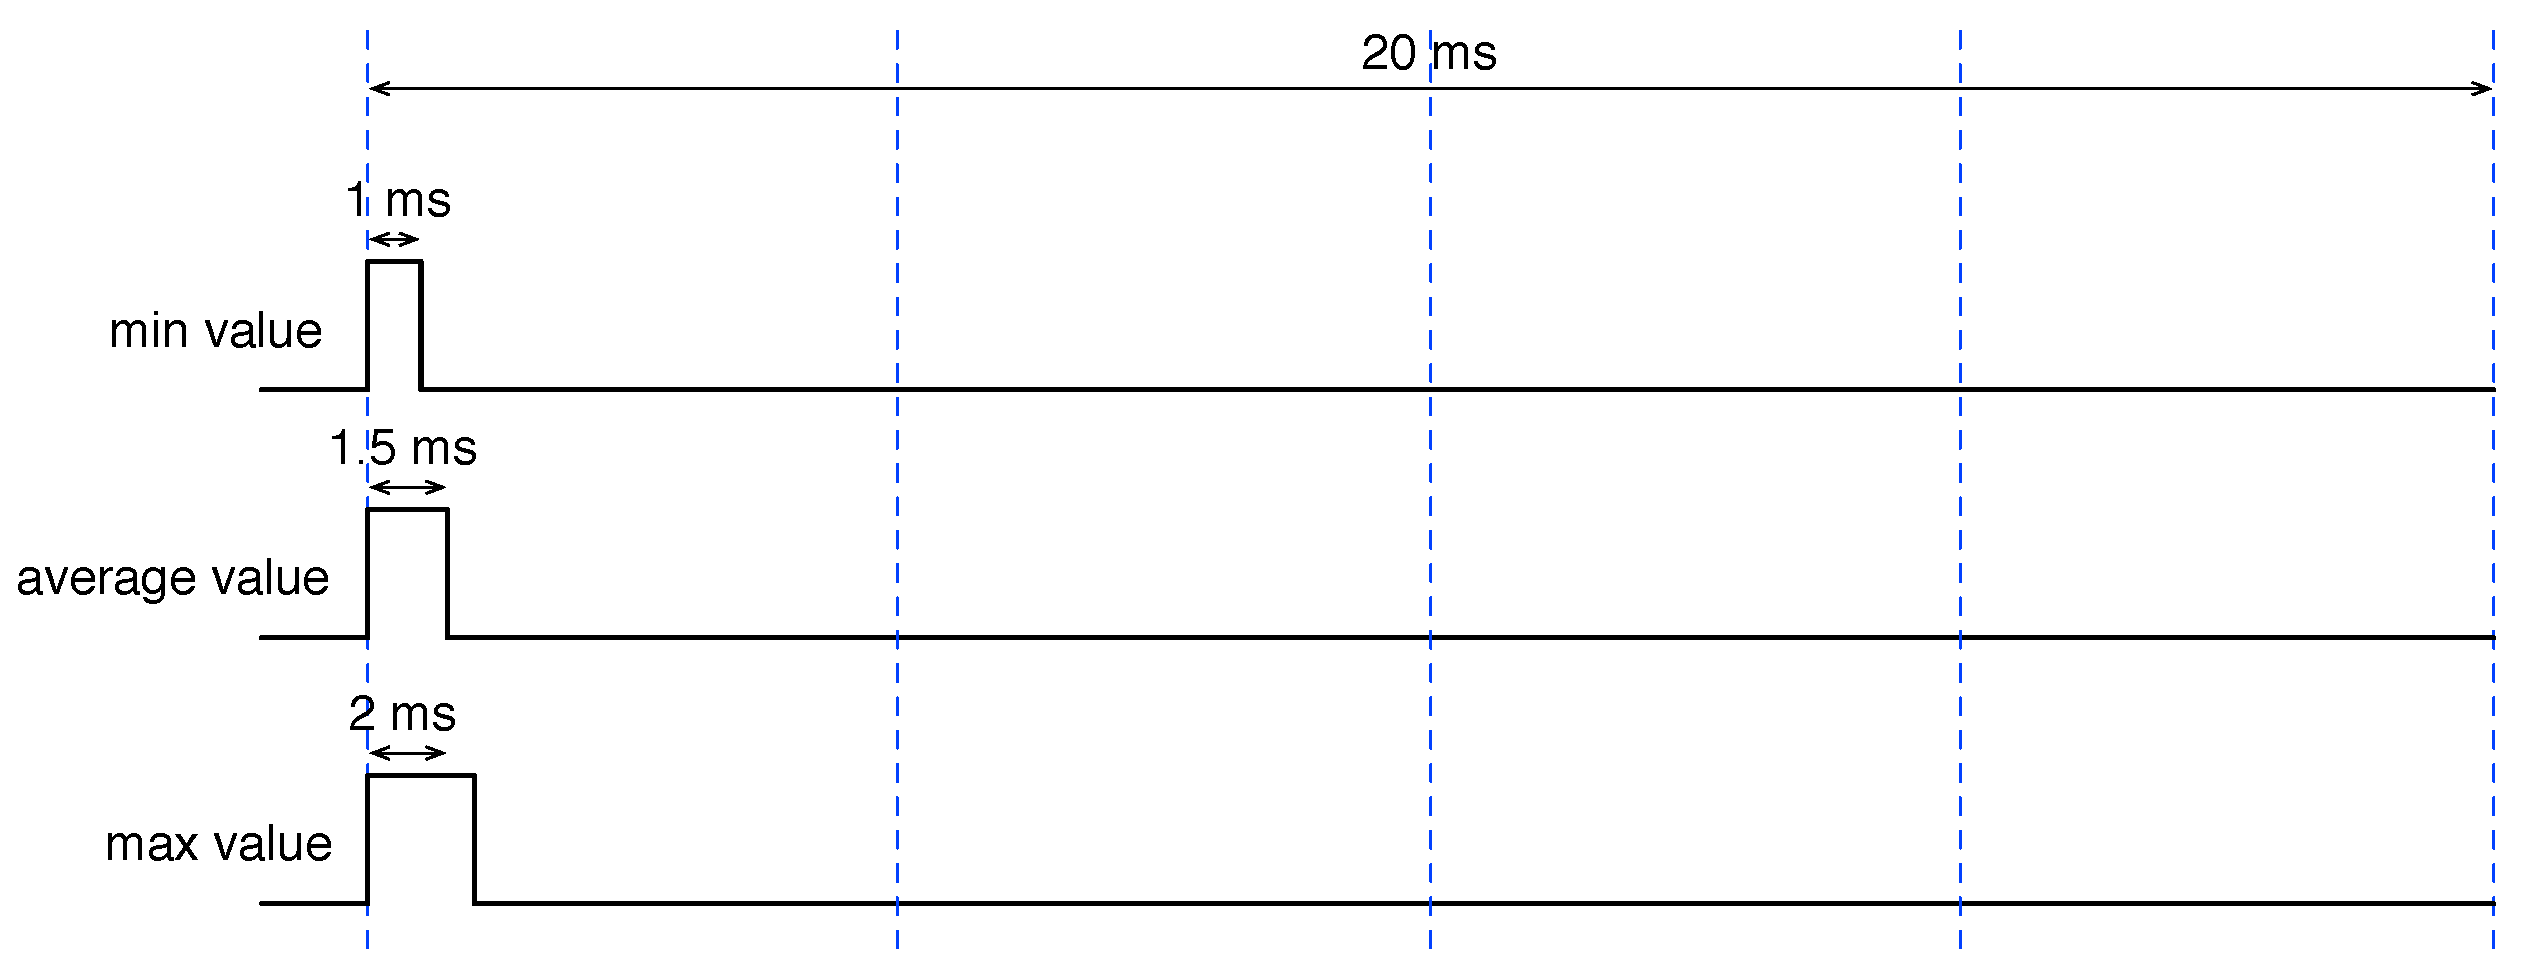
\includegraphics[width=\textwidth]{img/servopwm.pdf}
%
%\section{Servo PWM generation}
%
%The board has a 3 pins connectors for servos on the back side between the external power supply connector and the pair of white JST connectors. There is one symbol per pin: $-$, $+$ and \tikz[x=.5em,y=.5em]{\draw (0,0) -- ++(.5,0) -- ++(0,1) -- ++(1,0) -- ++(0,-1) -- ++(.5,0);}. The Servos must be connected with the {\bf yellow wire} on the \tikz[x=.5em,y=.5em]{\draw (0,0) -- ++(.5,0) -- ++(0,1) -- ++(1,0) -- ++(0,-1) -- ++(.5,0);} pin and the {\bf black wire} on the $-$ pin. as shown on the picture below.
%
%\begin{center}
%   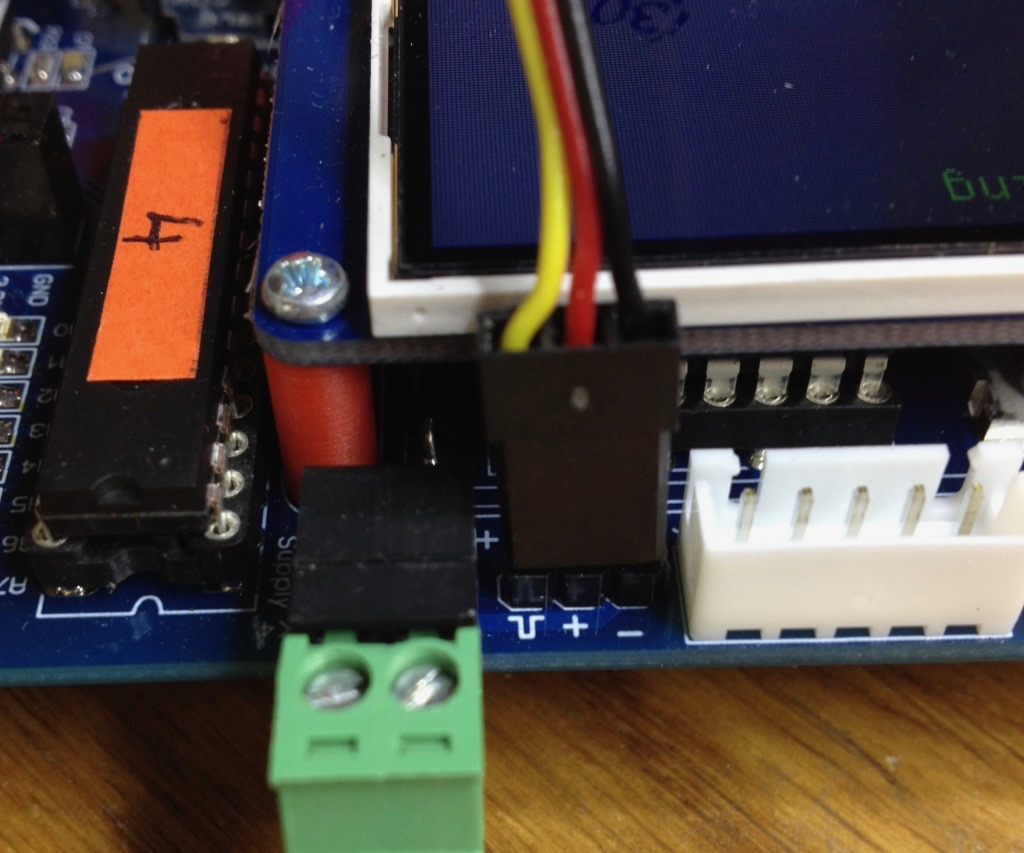
\includegraphics[scale=0.25]{img/servoconnection.jpg}
%\end{center}
%
%The 3.3V regulator of the Nucleo BB is not able to power the servo. We need an external power supply connected to the black power supply connector on the back of the board. Get a power supply cord and connect it to the power supply (9V) and to the board.
%
%We are going to drive 1 servo with a task named \texttt{t_servo}.
%
%\begin{ex}
%Program task \texttt{t_servo}. \texttt{t_servo} is periodic with a 20ms period. \texttt{t_servo} toggles the green LED, D1 (D3) (PORTB 0\footnote{Use digitalToggle(PORTB, 0).}). Verify the period using the scope\footnote{Plug a wire from the ground of the probe into the leftmost black connector terminal (labelled GND) and touch the LED left terminal with the probe.}.
%\end{ex}
%
%
%Now instead of toggling the LED, \texttt{t_servo} will use the function \texttt{setServoPulse}. This function takes 1 argument, the \texttt{duration} of the pulse in $\mu$s.  \texttt{setServoPulse} does not allow values lower than 1000 and greater than 2000 in order to avoid to damage the servo. \texttt{setServoPulse} works as follow: the \texttt{ouput} is set to 1 and a timer of the microcontroller is programmed to generate an interrupt after \texttt{duration} $\mu$s. In your OIL file, an ISR which is located in the \texttt{servo.c} file is defined as follow:
%
%\begin{lstlisting}
%  ISR isr_timer_7 {
%    CATEGORY = 1;
%    PRIORITY = 10;
%    SOURCE = TIM7_IRQ;
%  };
%\end{lstlisting}
%
%\begin{ex}
%Modify \texttt{t_servo} to use \texttt{setServoPulse} and generate a pulse with a width  equal to 1.5ms. Verify the behavior using the scope\footnote{Plug a wire from the ground of the probe into the leftmost black connector terminal (labelled GND) and touch \tikz[x=.5em,y=.5em]{\draw (0,0) -- ++(.5,0) -- ++(0,1) -- ++(1,0) -- ++(0,-1) -- ++(.5,0);} pin with the probe.}.
%\end{ex}
%
%Then connect the servo, it should go to the average position.
%
%\section{Adding high level behavior}
%
%Now we want to set the position of the servo. To do that we need 1 more task that sets the position in a global variable. The corresponding variable is read by the \texttt{t_servo} task to drive the servo.
%
%\begin{ex}
%First we want the position of the servo incremented until it reaches its maximum
%position (2ms pulse), then decremented until it reaches its minimum position
%(1ms pulse). So the servo does round trips. The time to go from the
%minimum position to the maximum position is 5s. Assuming the position is
%incremented and decremented by one, what is the period of this task in
%counter tick unit?
%Program the resulting application.
%\end{ex}
%
%Now we want to be able to set the minimum and maximum positions of the servo. To do that we use buttons.
%
%\begin{ex}
%Add to the previous application the following features and draw an automaton to model the application:
%
%When button B4 is pressed, the servo stops its round-trip. Then (when round-trip is stopped), the following functions are available:
%
%When DIP switch B0 is ON, the minimum position is selected, the servo goes to this position. Then push buttons B7 decrements the minimum position and B5 increments the minimum position.
%
%When DIP switch B0 is OFF, the maximum position is selected, the servo goes to this position. Then push buttons B7 decrements the maximum position and B5 increments the maximum position.
%
%Minimum position should be kept greater than or equal to the position corresponding to the 1ms pulse. Maximum position should be kept lower than or equal to the position corresponding to the 2ms pulse. Minimum position should be kept lower than or equal to the maximum position.
%
%When button B4 is pressed again, the servo resumes its round-trip within the minimum and maximum positions that have been set.
%
%\end{ex}

\end{document}
